\documentclass[english,ngerman,parskip=half]{scrartcl}
\usepackage{amsmath}
\usepackage{amssymb}
\usepackage{amsthm}
%\usepackage[portuges]{babel}
\usepackage[utf8]{inputenc}
\usepackage{graphicx}
\usepackage[T1]{fontenc}
\usepackage{systeme}
\newcommand{\abs}[1]{\lvert #1 \rvert}

%\usepackage{libertine}
\usepackage{microtype}
\usepackage{lmodern}
\usepackage[brazilian]{babel}
\usepackage{xcolor}


\begin{document}
 %capa copiada de https://tex.stackexchange.com/questions/177283/create-a-cover-for-my-thesis
 %start Cover

    \begin{titlepage}
        \vspace*{-3cm}
        %\makebox[\dimexpr\textwidth+2cm][r]{\includegraphics[height=1.5cm]{FULogoRGB(1)}} 
        \makebox[\dimexpr\textwidth+2cm][r]{
\includegraphics[height=1.5cm]{./images/marca-udesc.png}} 

        \vspace*{5cm}
    \begin{center}
        \Huge\bfseries\sffamily Trabalho de cálculo II

        \vspace*{2cm}
        \large 
        Silva

        Mateus Schroeder da
    \end{center}

    \enlargethispage{3cm}
    \vfill
    \parbox[t]{0.45\textwidth}{%
            %Matrikelnummer: 1234572              \\
                Área: Matemática \\
                    Universidade: UDESC/CCT \\
                    {\selectlanguage{brazilian}\today}
                          }%
                          \hfill
                          \begin{tabular}[t]{l@{}}%{\raggedleft%
                              Professor:\\
                                Dr. Elizandra Bar de Figueiredo
                              \end{tabular}
                              %}%
                          \end{titlepage}
% end Cover

\begin{enumerate}
    %%%%%%%%%% Exercício 1 - Início
    \item
        Vamos encontrar um parabolóide que satisfaça a condição exigida.
        Sabendo que um parabolóide qualquer pode ser expresso por:
        $$ p: c_1 \cdot \left( x - a \right)^2 + c_2 \cdot \left( y - b\right)^2 + d = z$$
        Onde $c_1, c_2, a, b \in \mathbb{R} \land c_1 \cdot c_2 > 0$ \\
        Com a equação do plano dada: $ \pi: 13x - 8y - z = 24 \iff 13x -8y -24 = z$ podemos obter o vetor normal, 
        $\overrightarrow{n} = (-13, +8, +1)$. 

        \systeme*{{-13 = -\dfrac{\partial f}{\partial x} (1,2)},,{+8 = -\dfrac{\partial f}{\partial y} (1,2)}}
        $$ -13 = -\dfrac{\partial f}{\partial x} (1,2) \implies 2c_1 - 2c_1a = +13$$
        $$ +8 = -\dfrac{\partial f}{\partial y} (1,2) \implies 4c_2 - 2c_2b = -8$$
        Substituindo com qualquer par de números reais tais que $c_1 \cdot c_2 > 0$, escolheremos $c_1 = 3$ e $c_2 = 7$ então:
        $$ 2 \cdot 3 - 2 \cdot 3 \cdot a = 13 \implies a = \dfrac{-7}{6}$$
        $$ 4 \cdot 7 - 2 \cdot 7 \cdot b = -8 \implies b = \dfrac{18}{7}$$
        E assim temos a equação:
        $$ 3 \left( x + \dfrac{7}{6} \right)^2 + 7 \left( y - \dfrac{18}{7} \right)^2 + d = z $$
        E para encontrar $d$ basta substituir as variáveis da equação no ponto que desejamos que pertença a esse parabolóide.
        Então segue:
        $$ 3 \left( 1 + \dfrac{7}{6} \right)^2 + 7 \left( 2 - \dfrac{18}{7} \right)^2 + d = -27 $$
        $$ \dfrac{169}{12} +\dfrac{16}{7} + d = -27 \implies d = \dfrac{-3643}{84}$$
        Temos agora a equação que procurávamos, que é dada por:
        $$ 3 \left( x + \dfrac{7}{6} \right)^2 + 7 \left( y - \dfrac{18}{7} \right)^2 -\dfrac{3643}{84} = z $$
        A figura está representada abaixo na figura \ref{exercicio1}:
        \begin{figure}[ht!]
            \centering
            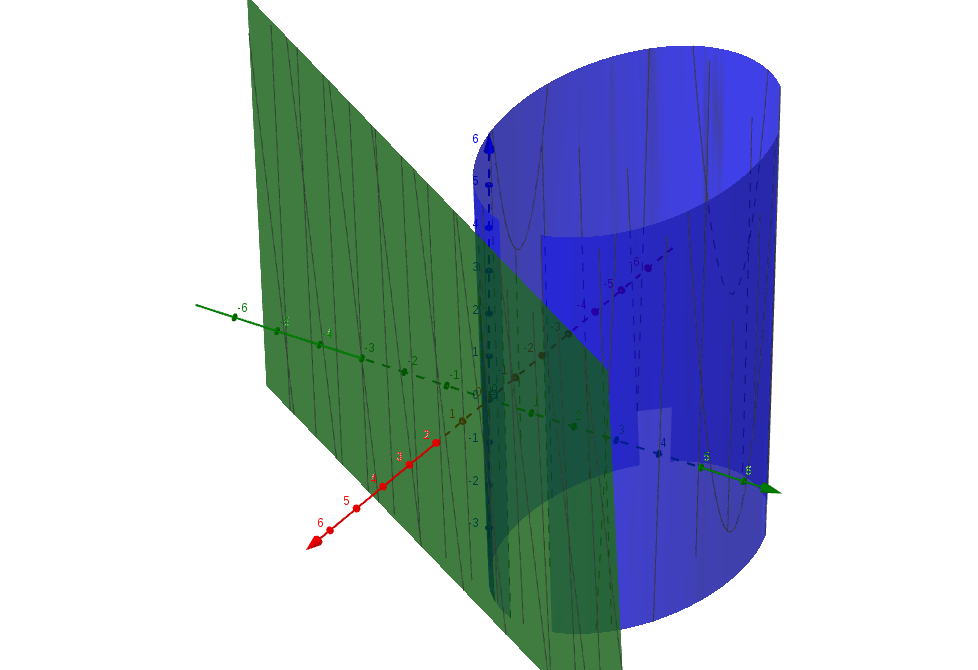
\includegraphics[width=90mm]{./images/exercicio1.png}
            \caption{Plano e parabolóide\label{exercicio1}}
        \end{figure}
\newpage
    %%%%%%%%%% Exercício 1 - Fim

    %%%%%%%% Exercício 2 - Início
    \item
        Vamos chamar o sólido por corneta. 
        Ela é representada na figura \ref{solido}:

        \begin{figure}[ht!]
            \centering
            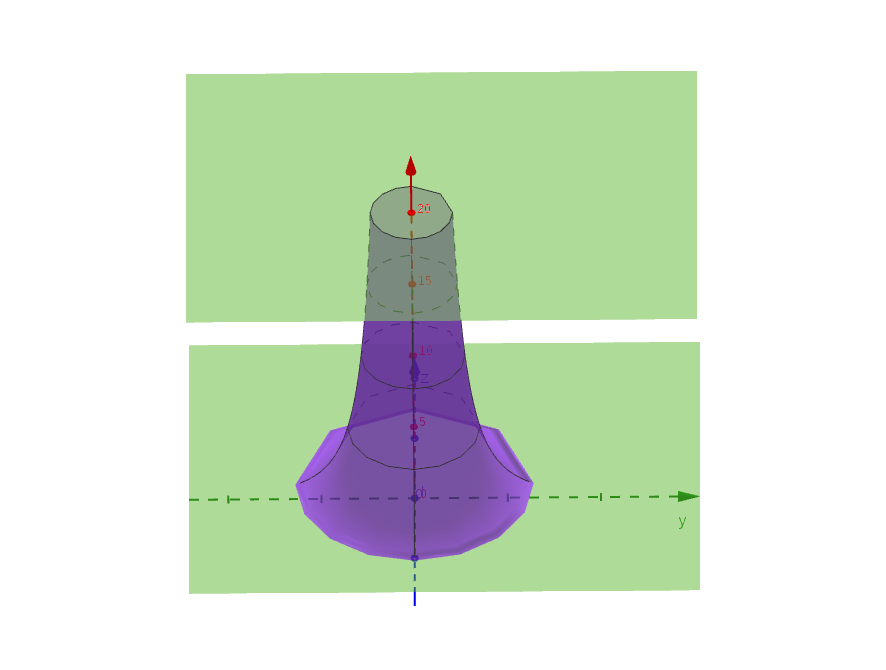
\includegraphics[width=90mm]{./images/3d-solido.png}
            \caption{Corneta \label{solido}}
        \end{figure}
        
        Construiremos o sólido tem torno do eixo $x$.
        A figura é delimitada por dois planos, a saber $x = 1$ e $x = 20$. \\
        Chamando \\
        $
        d_1 = 1 , \\
        d_2 = 5 + d_1 = 6, \\
        d_3 = 5 + d_2 = 11, \\
        d_4 = 5 + d_3 = 16, \\
        d_5 = 4 + d_3 = 20$ \\
        Seja $I_n = \{x \in \mathbb{N}; x \leq n\}$ \\
        Tomando os planos $p_n: x = d_n, n \in I_5$ temos eles 
        representados abaixo na figura \ref{3d-planos-dn}:

        \begin{figure}[ht!]
            \centering
            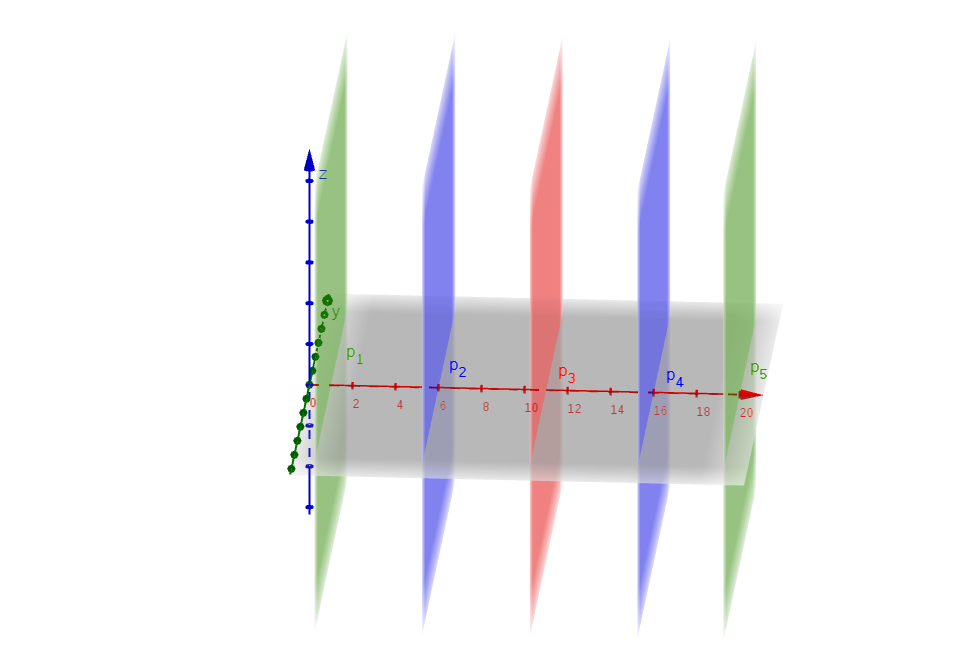
\includegraphics[width=90mm]{./images/3d-planos-dn.png}
            \caption{Planos definidos por $d_n$ \label{3d-planos-dn}}
        \end{figure}
    
        Sejam então os raios aproximados das mensurações (os denominadores representam o diâmetro): \\
        $$ r_1 = \dfrac{13}{2} \approx 6.5,$$ 
        $$ r_2 = \displaystyle \dfrac{7}{2} \approx 3.5, $$
        $$r_3 = \dfrac{6}{2} \approx 3,$$
        $$r_4 = \dfrac{4.7}{2} \approx 2.35,$$
        $$r_5 = \dfrac{4.5}{2} \approx 2.25$$

        Essas circunferências foram obtidas da seguinte forma:
        $$c_n: x = d_n  \land r_n^2 = y^2 + z^2 \implies x = d_n = \dfrac{d_n}{r_n^2} \cdot \left( y^2 + z^2 \right)$$
        Então fazemos a interseção da circunferência com o plano $xy$, que nos 
        fornecerá os pontos $A_n, B_n, ..., E_n$ como mostra a figura \ref{3d-intersecao-circ-xy}:

        \begin{figure}[ht!]
            \centering
            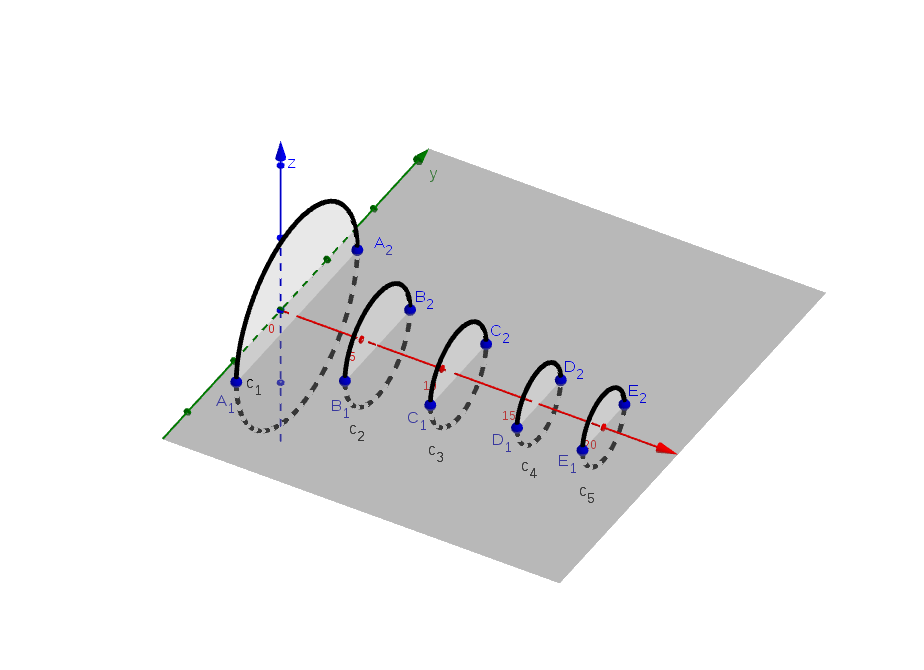
\includegraphics[width=90mm]{./images/3d-intersecao-circ-xy.png}
            \caption{Interseção das circunferências com o plano $xy$ \label{3d-intersecao-circ-xy}}
        \end{figure}

        Consequentemente, no plano $xy$ os pontos são mostrados na figura \ref{figu}:

        \begin{figure}[ht!]
            \centering
            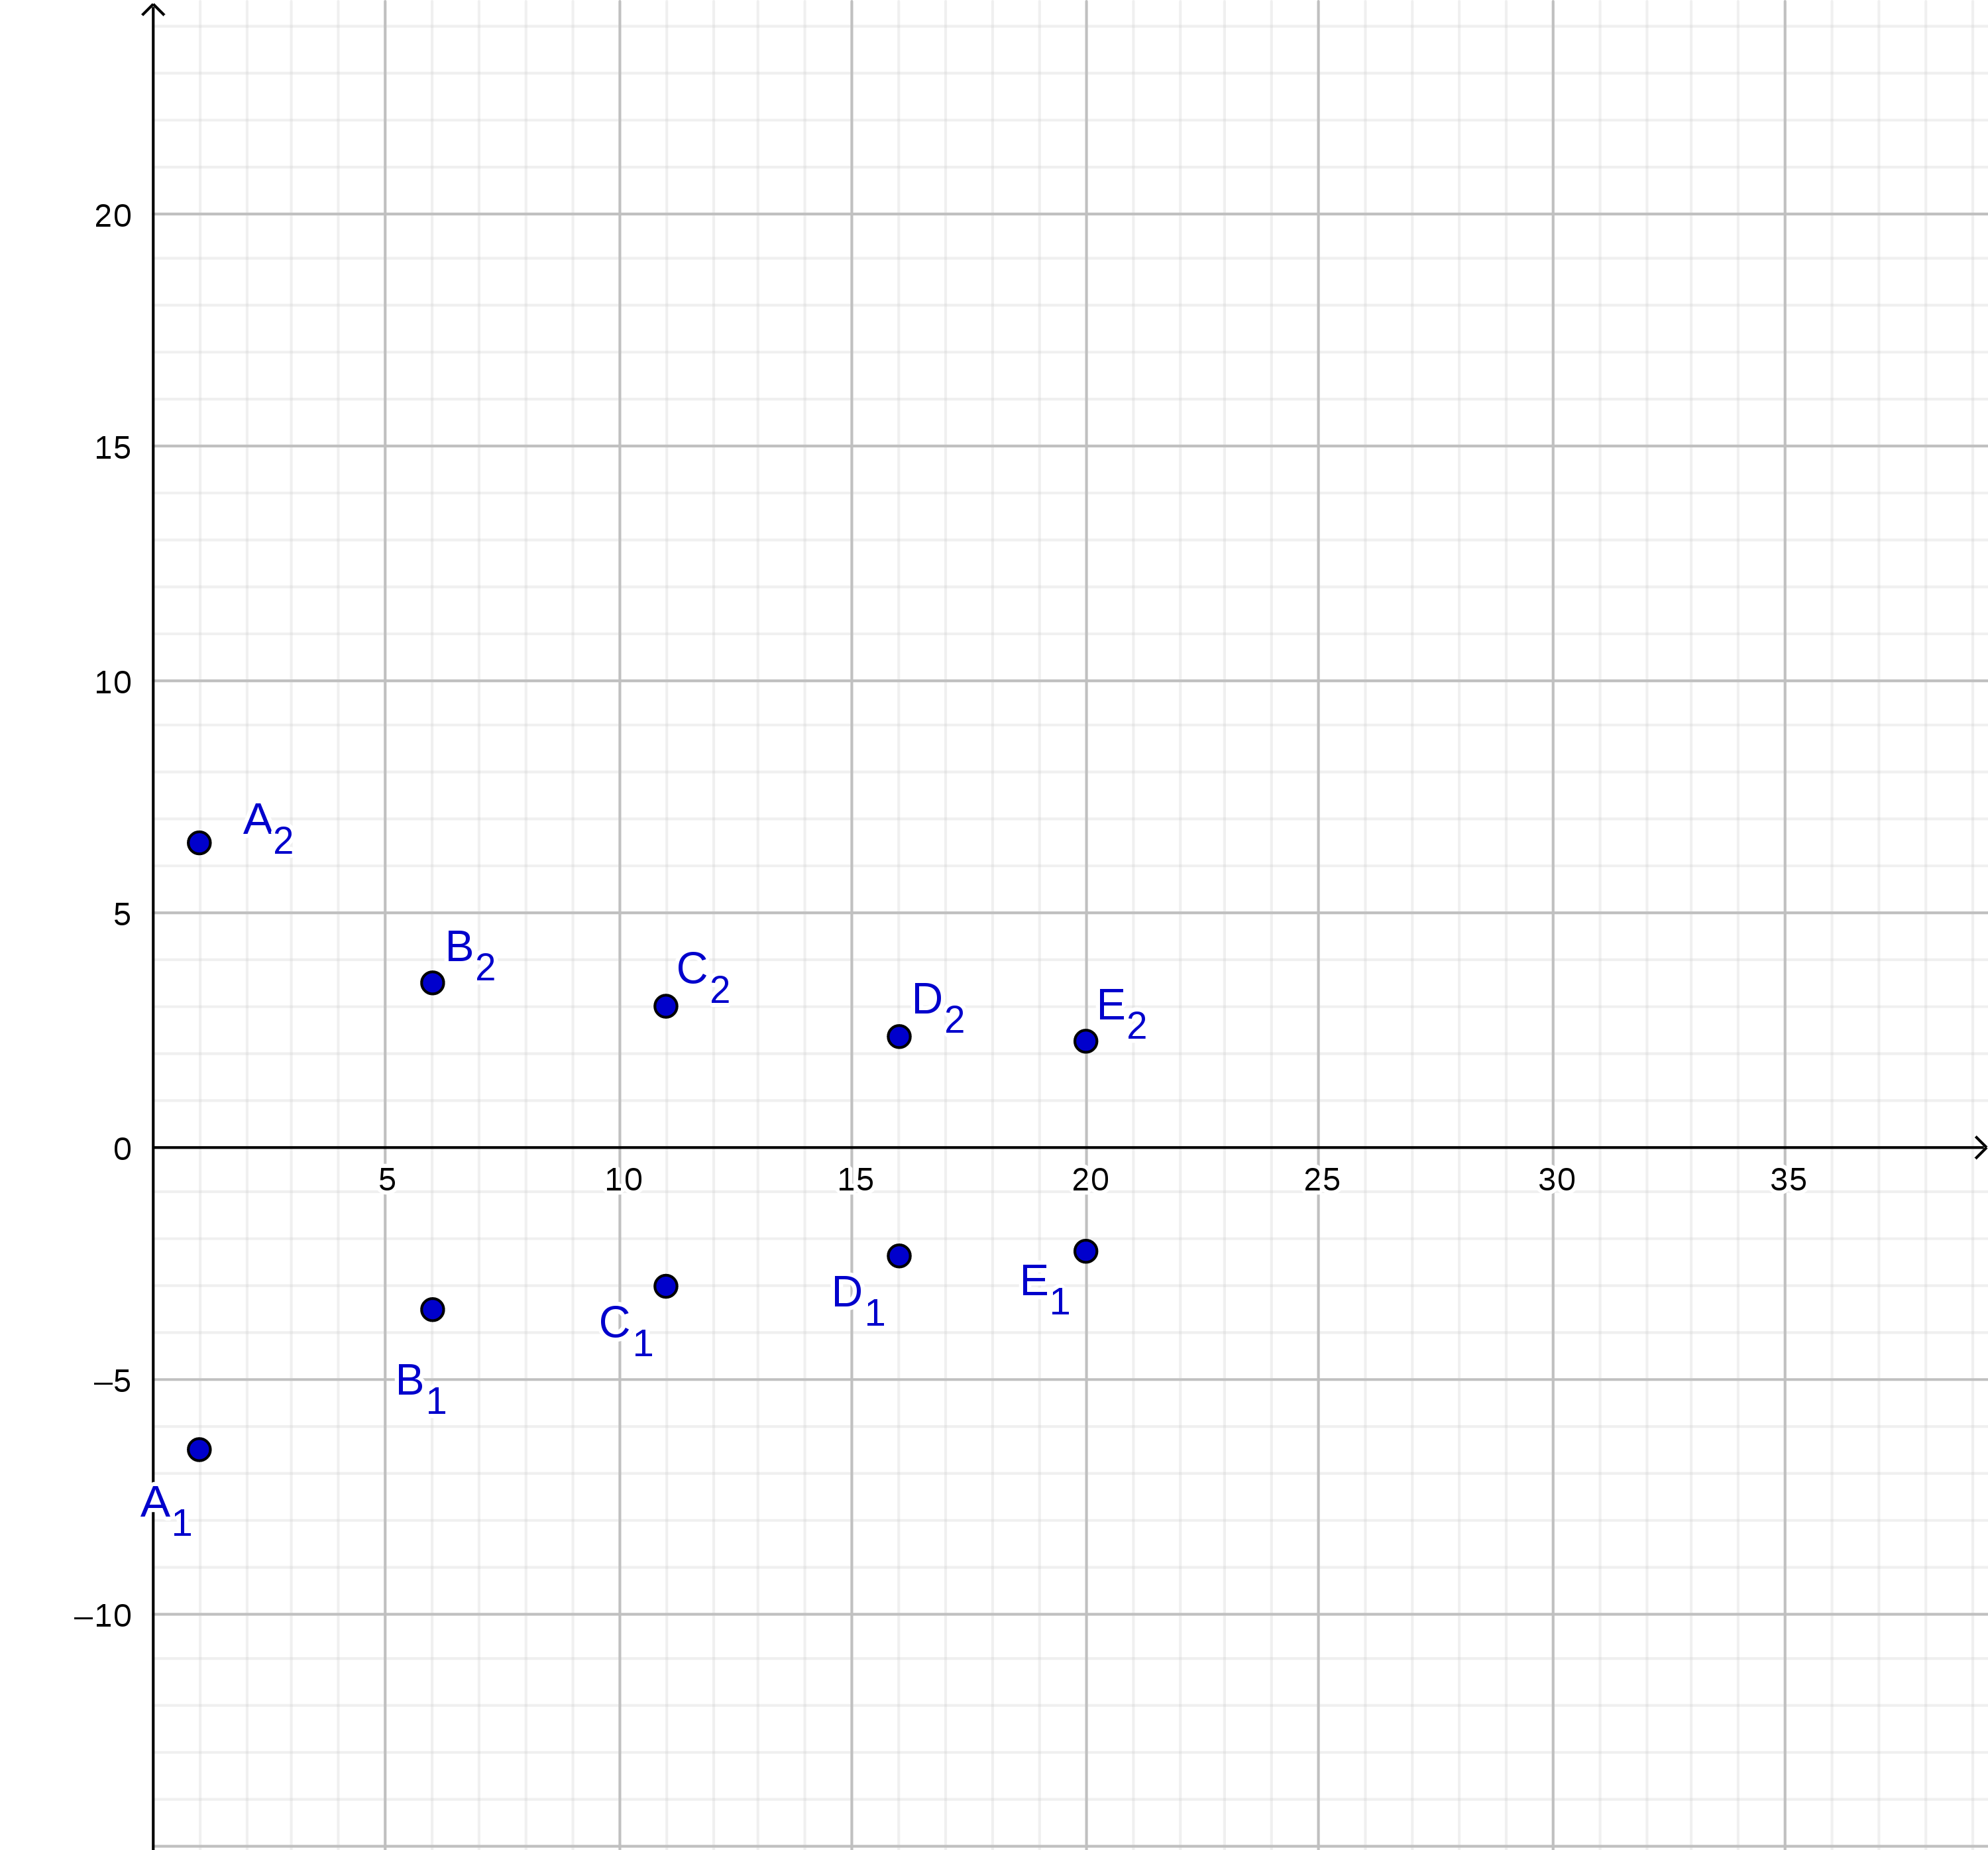
\includegraphics[width=90mm]{./images/2d-intersecao-circ-xy.png}
            \caption{Interseção das circunferências com o plano $xy$}
            \label{figu}
        \end{figure}

        Na tentativa de encontrar uma função derivável (porque a corneta "é derivável")
        que atinja aproximadamente os pontos encontrados, sugerimos primeiramente:
        $$ f(x) = \dfrac{1}{x}$$
        E posteriormente:
        $$ f(x) = \dfrac{a}{x^c} + b$$
        Com $a,b,c \in \mathbb{R}$.
        Utilizando os "sliders" do Geogebra, nos permite aproximar a corneta com 
        $$ f(x) = \dfrac{6}{x^{0.4}} + 0.4$$
        
        \begin{figure}[ht!]
            \centering
            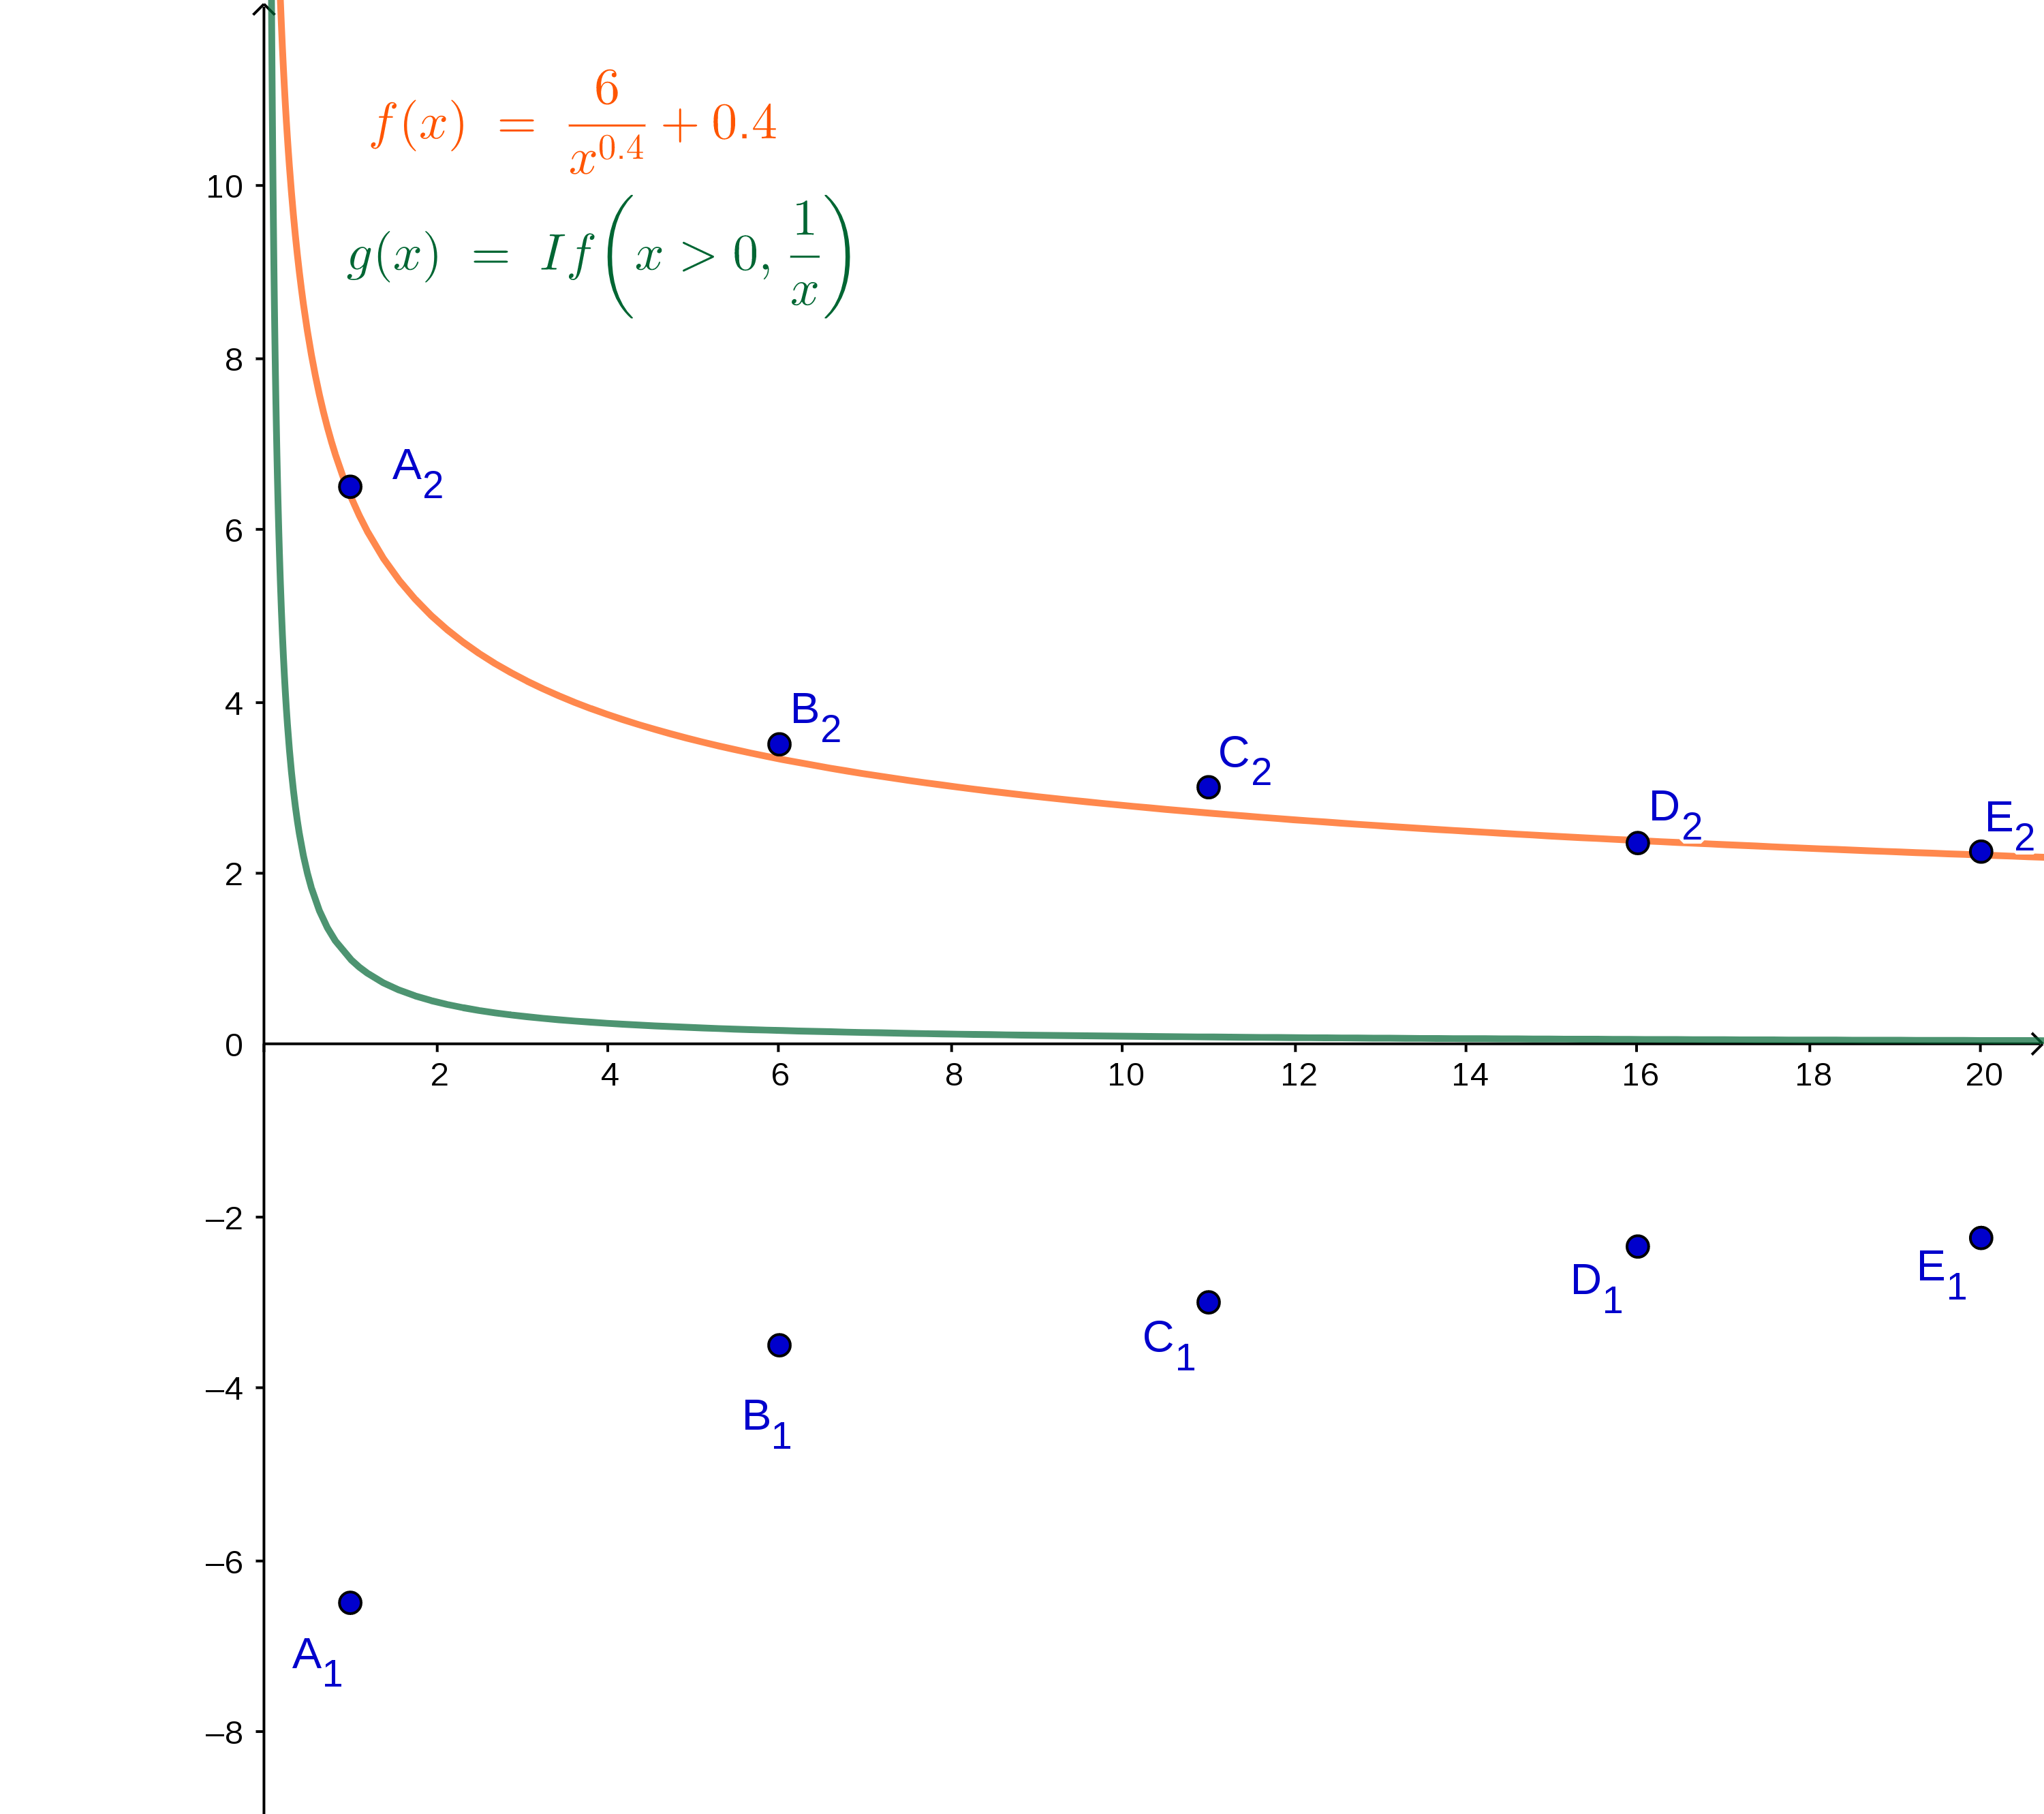
\includegraphics[width=90mm]{./images/2d-x-na-menos-um-e-aproximacao.png}
            \caption{Aproximando os pontos com função \label{2d-x-na-menos-um-e-aproximacao}}
        \end{figure}
        

        Por fim, basta limitar $f(x)$ no domínio e rotacionar usando o comando "surface", então obtemos:
        
        \begin{figure}[ht!]
            \centering
            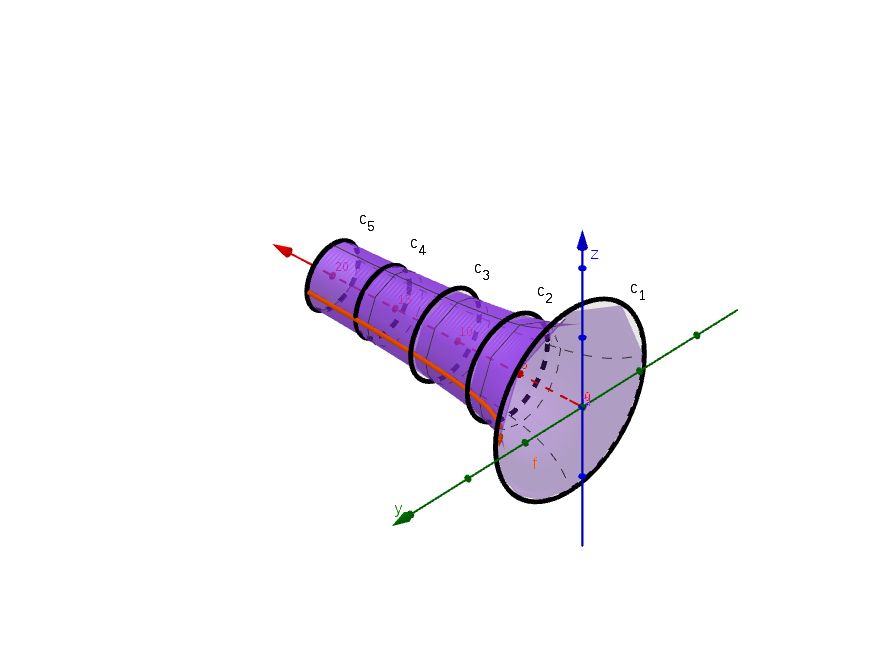
\includegraphics[width=90mm]{./images/3d-solido-pronto-e-funcao-geradora.png}
            \caption{Sólido, função geradora, circunferências \label{3d-solido-funcao-circunferencias}}
        \end{figure}

        
        Para obtermos o volume do sólido, temos:
        $$ V = \pi \int_a^b[f(x)]^2 dx = \int_1^{20} \dfrac{6}{x^{0.4}} + 0.4 dx$$
        $$ \int \dfrac{6}{x^{0,4}} + 0,4 dx = 0,4x + 10 x^{0,6} $$
        $$ V = F(20) - F(1) = (0,4 \cdot 20 + 10 \cdot 20^{0,6}) - (0,4 + 10) \approx 57,94 u.v.$$
        
    %%%%%%%% Exercício 2 - Fim 

     %%%%%%%% Exercicio 3 - Início
    \item 
        \begin{enumerate}
            \item Se Leonard consegue  dar passos que atendem ao método de Zenão (ou Zeno), então talvez seja
                possível que 
                ele consiga também dar uma quantidade infinita de passos. Mas se ele não consegue 
                dar infinitos passos, então ele não consegue atravessar o corredor utilizando o método de Zenão.
                Mas suponhamos que os cinco primeiros passos ele utilize do método de Zenão, então no quinto passo
                ele estará $\approx 1,2m$ distante, e quem dá um passo de $19m$ dá um passo de $2$ então ele atravessa.
            \item
                O corredor tem $d = 38.50m$ então, \\
                Primeiro passo: $19.25m$ \\
                Segundo passo: $28.875m$ 
            \item 
                \begin{align*}
                    d_1 &= \dfrac{d}{2^1} = 19,25\\
                    d_2 &= \dfrac{d}{2^1} + \dfrac{d}{2^2} \approx 28,87 \\
                    d_3 &= \dfrac{d}{2^1} + \dfrac{d}{2^2} + \dfrac{d}{2^3} \approx 33,68 \\
                    d_4 &= \dfrac{d}{2^1} + \dfrac{d}{2^2} + \dfrac{d}{2^3} + \dfrac{d}{2^4} \approx 36,09 \\
                    d_5 &= \dfrac{d}{2^1} + \dfrac{d}{2^2} + \dfrac{d}{2^3} + \dfrac{d}{2^4} + \dfrac{d}{2^5} \approx 37,29 \\
                    \\
                    d_n &= \dfrac{d}{2^1} + \dfrac{d}{2^2} + \dfrac{d}{2^3} + \hdots + \dfrac{d}{2^n} \\
                        &= d \cdot \sum_{i=1}^n 2^{-i} \\
                        &= 38,50 \cdot \sum_{i=1}^n 2^{-i} 
                \end{align*}
            \item
                Se as fórmulas que seguem representam o problema (com somas infinitas não se brinca, disseram), então sim.
                $$ 38,50 - 38,50 \sum_{i=1}^n 2^{-i} < 38,50 \epsilon \iff 1 - \sum_{i=1}^n 2^{-i} < \epsilon $$
                Dado um $\epsilon$ qualquer, vamos escolher um novo e chamá-lo pelo mesmo símbolo, 
                tal que é o maior $2^{-k}$ que seja menor que o $\epsilon$ anterior, com $k$ natural.
                Vamos provar para todo $\epsilon$ dado existe $n$ tal que vale:
                $$1 < \sum_{i=1}^n 2^{-i} + \epsilon $$
                \begin{proof}
                Tomando $n = k+1$, por indução sobre $k$ se $k = 1$:
                $$\sum_{i=1}^{k+1} 2^{-i} + \dfrac{1}{2^k} =
                    \sum_{i=1}^{1+1} 2^{-i} + \dfrac{1}{2^1} =
                    \dfrac{1}{2^1} + \dfrac{1}{2^2} + \dfrac{1}{2^1} > 1 $$
                Nossa hipótese de indução é que existe um $k_0 = k$ tal que:
                $$ \sum_{i=1}^{k+1} 2^{-i} + \dfrac{1}{2^k} > 1$$ 
                Provemos que vale também para $k+1$
                \begin{align*}
                    & \sum_{i=1}^{(k+1)+1} 2^{-i} + \dfrac{1}{2^{(k+1)}} = \\
                    %& \sum_{i=1}^{k} 2^{-i} + \dfrac{1}{2^{k+1}} + \dfrac{1}{2^{k+2}} + \dfrac{1}{2^{(k+1)}} = \\
                    & \sum_{i=1}^{k} 2^{-i}\dfrac{1}{2^{k+1}} + \dfrac{1}{2^{k+2}} + \dfrac{1}{2^{(k+1)}} = \\
                    & \left( \sum_{i=1}^{k} 2^{-i} \dfrac{2 \cdot 1}{2^{k+1}} \right) + \dfrac{1}{2^{k+2}}  > 1
                \end{align*}
                \end{proof}
            \item
                Se ele fosse dando um passo após o outro, ele chega cada vez mais próximo, até o momento em que ele para de 
                andar com o método de Zenão e dá um passo que chega no final do corredor ou o atravessa.
            \item
                $$ 38,50 - 38,50 \sum_{i=1}^n 2^{-i} $$
                Desconsiderando a subtração, a primeira parcela da soma é a distância a percorrer e a 
                segunda é o passo $n$ que pode ser entendida como
                uma função na variável $d$.
                No exercício (d) mostramos que Leonard pode aproximar-se arbitrariamente do final do corredor tanto quanto
                se queira. Isso pode ser representado dizendo que o limite das somas parciais da série cujos termos são 
                os tamanhos dos passos é convergente, e "converge para o fim do corredor".
                Note que também pode ser argumentado que a série é um múltiplo da série geométrica com base menor que 1.
        \end{enumerate}
        %%%%%%%%%%% Exercicio 3 - Fim  
\end{enumerate}
%\begin{enumerate}
%    %\item
%        %Primeiro consideraremos algumas fórmulas antes de começar a dedução.
%        %$ d(P_i, P_{i-1}) = \sqrt{ 1+ f'(x_i^*} \cdot \Delta x $ onde $x^*$ é algum ponto do domínio de $f$ \\
%        %$ A_l = 2\pi g$
%        %onde $r$ é $ (raio maior + raio menor)/2$ e $g$ é a geratriz do tronco de cone.
%%
%        %Deduziremos a fórmula de uma função $f$ que é contínua.
%%
%        %A ideia é considerar o limite quando $\Delta x \rightarrow 0$ e calcular a área do tronco de cone.
%%
%        %Consideraremos $P_j$ pontos da curva que será feita revolução.
%%
%        %$$f(x_i) \approx f(x_i^*) \approx f(x_{i-1}) $$
%        %$$A_i = 2\pi \left( \dfrac{ f(x_i) + f(x_{i-1} }{2} \right) \cdot d(P_i, P_{i-1}) \approx $$
%
%
%    \item
%    Considerando a função
%    $$ f(x,y) = \dfrac{(x-1)^2 + x(y+1)^2} {(x-1)^2+(y+1)^2}$$
%    primeiramente vamos pegar um $\epsilon$ “qualquer” (considerando as capacidades 
%    do Geogebra) usando o “slider”, que nesta atividade está variando de $0.1$
%    até $0.5$. 
%    
%    Sabendo que o limite da função quando $f \rightarrow (1,-1)$ é igual a 1, temos pela definição de limite:
%    $\abs{ f(x,y) - 1 } < \epsilon  \iff -\epsilon + 1 < f(x,y) < \epsilon + 1$
%    Se considerarmos $-\epsilon+1$ e $\epsilon + 1$ como a terceira coordenada de um
%    plano cada um, temos que $\epsilon + 1$ é o plano verde, e $- \epsilon + 1$
%    é o plano amarelado na figura abaixo.
%
%    \begin{figure}[ht!]
%        \centering
%        \includegraphics[width=90mm]{img1.png}
%        \caption{Intersecção e projeção no plano $xy$ \label{intersecao}}
%    \end{figure}
%
%    Ainda considerando a Figura \ref{intersecao}, temos em roxo o gráfico de $f$, também as
%    intersecções de $f$ com os planos, e a translação da intersecção de $f$ com os planos, no plano $xy$.
%    A reta preta que passa por $A$ é uma reta perpendicular a $xy$.
%    
%    \newpage
%    \begin{figure}[ht!]
%        \centering
%        \includegraphics[width=90mm]{img2.png}
%        \caption{Projeção da intersecção \label{projecao}}
%    \end{figure}
%    Na figura \ref{projecao}, temos a translação das interseções dos planos com $f$ no plano
%    $xy$, que estão de cores verde e amarelo. Tem-se então que há duas distâncias, do 
%    ponto $A$ até a translação amarela, e outra de $A$ até a translação verde. 
%    Pegando a menor delas, conseguimos fazer como na Figura
%    \ref{imagem_entre_planos}, a seguir, onde todo
%    o gráfico de $f$, restrito ao círculo (aberto) preto, está entre os planos verde e amarelo.
%    \begin{figure}[ht!]
%        \centering
%        \includegraphics[width=90mm]{img3.png}
%        \caption{Imagem de $f$ entre os planos $\epsilon+1$ e $-\epsilon + 1$
%        \label{imagem_entre_planos}}
%    \end{figure}
%    \item
%        Consideraremos a função 
%        $$ f(x,y) = x^2y^2 , x\neq 0 \neq y$$
%        Sejam 
%        $$\pi_1: y=1$$ 
%        $$ C_1 = \pi_1 \cap f $$
%        Temos 
%        \begin{equation}
%           C_1: y=1 \land x^2y^2=z \iff C_1: x^2=z, y=1
%        \end{equation}
%        $C_1$ é a interseção de $f$ com $\pi_1$ e sua derivada parcial, que nos
%        dá o valor do ângulo da reta tangente em cada um de seus pontos é dada
%        por:
%        $$ \dfrac{\partial y^2x^2}{\partial x} = y^22x \leadsto 1\cdot2\cdot
%        (-1) = -2$$
%        Portanto $-2$ é o valor do ângulo da reta tangente à $C_1$ considerando
%        o eixo de referência $z=0, y=1, x=x$.
%
%        De (1) temos a equação de $C_1$ e sua derivada parcial no ponto $(-1,1)$. Agora queremos
%        descobrir a reta $r_1$ tangente à $C_1$.
%        
%        Pelo desenvolvimento, ocorre $r_1 \subset \pi_1$, pois $$( \pi_1 \cap f)
%        \subset\pi_1 $$ e portantanto, a derivada de uma curva do plano, se existir, estará contida no plano.
%
%        Conseguimos determinar que $r_1 \subset \pi_1$, agora prossigamos com a
%        fórmula da reta no plano:
%        $$ z - z_0 = \alpha ( x - x_0) \iff
%        z - f(x_0,y_0) = \dfrac{\partial f(-1,1)}{\partial x} \cdot (x-x_0) $$
%        que substituindo os valores temos:
%        $$ z - 1 = -2\left(x-(-1)\right) \iff z = -2x-1 $$
%        Então temos que $r_1: y=1 \land z=-2x-1$
%
%        Analogamente encontramos $C_2$ e $r_2$, que são:
%        $$ C_2: z=y^2$$
%        $$r_2: x=-1 \land z=y^2$$
%
%        Sabendo que duas retas concorrentes determinam um único plano, e sabendo
%        que o vetor normal de um plano é dado pelo produto vetorial de quaisquer
%        dois vetores não múltiplos entre si, temos:
%
%        $$\overrightarrow{\rm n_{\pi}} = \overrightarrow{\rm v_1} \times
%        \overrightarrow{\rm v_2}$$
%        onde $\overrightarrow{\rm v_1}$ e $\overrightarrow{\rm v_2}$ são vetores
%        diretores de $r_1$ e $r_2$, e $\pi$ é o plano tangente no ponto
%        considerado. E ainda, desconsideramos que o vetor normal não é
%        único, mas este é um vetor normal e é suficiente.
%
%        Por brevidade, usaremos a fórmula para obter o vetor normal:
%        $$\overrightarrow{\rm n_{\pi}} = \left(- \dfrac{\partial f(-1,1)}{\partial x} ,
%        - \dfrac{\partial f(-1,1)}{\partial y},
%        1 \right)$$
%
%        Da equação geral do plano: $ax + by + cz + d = 0$, substituindo os
%        valores temos:
%        $$ 2(-1) -2(1) + 1(1) + d = 0 \implies d = 3$$
%        E a equação do plano tangente é:
%        $$ +2x - 2y +z + 3 = 0 $$
%        
%        A Figura \ref{plano_tangente} ilustra a função e o plano tangente:
%
%    \begin{figure}[ht!]
%        \centering
%        \includegraphics[width=90mm]{img4.png}
%        \caption{Plano tangente \label{plano_tangente}}
%    \end{figure}
%\end{enumerate}



\end{document}

